\documentclass{article}
\usepackage{amsmath}
\usepackage{ctex}
\usepackage{geometry}
\usepackage{lmodern}
\geometry{a4paper,scale=0.8}

\usepackage{algorithm}  
\usepackage{algpseudocode} 
\usepackage{enumerate}
\usepackage{graphicx}
\usepackage{subfigure}
\usepackage{float}
\floatname{algorithm}{算法}  
\renewcommand{\algorithmicrequire}{\textbf{输入:}}  
\renewcommand{\algorithmicensure}{\textbf{输出:}} 

\usepackage{pgf}
\usepackage{tikz}

\title{高级算法作业二}
\author{1190200122 袁野}
\date{2022年4月10日}
\setlength{\parindent}{0pt}
\begin{document}
\maketitle
\paragraph{2.1}~{}

(a)
设两个人的编号分别为$i$和$j$,那么就有
$$
\left\{
\begin{aligned}
    p(i) &= (i-10)\times s-(i-11)\times f \\
    p(j) &= (j-10)\times s-(j-11)\times f \\
\end{aligned}
\right.
$$
可以发现这是一个以$s$和$f$为未知数的二元一次方程组,联立求解即可得出$$s=\frac{(i-11)p(j)-(j-11)p(i)}{i-j}$$

(b)
对于第$i$个人来说,他只知道$p(i) = (i-10)\times s-(i-11)\times f$,这是一个二元一次函数,想要知道$s$的取值必须需要直到$f$的取值,
而$f \in GF(q)$,$q$是一个101位的素数,所以$f$有$2^{100}$种以上的取值,盲猜$f$的取值的话概率$p \le \frac{1}{2^{100}}$,
这是一个极小的取值,因此一个用户是无法得知$s$的。
\paragraph{2.2}~{}

$\bullet$ 首先证明$X_{ij}$两两独立:

任取$i,j,k,l$且满足$i<j,k<l$,需要证明$Pr(X_{ij}=x_1 \cap X_{kl}=x_2) = Pr(X_{ij}=x_1) \times Pr(X_{kl}=x_2) (x_1,x_2 \in {0,1}) $

当$i,j,k,l$互不相同时,该等式显然成立。

当$i,j,k,l$并不互不相同时,不妨设$i=k$,即证明$Pr(X_{ij}=x_1 \cap X_{il}=x_2) = Pr(X_{ij}=x_1) \times Pr(X_{il}=x_2) (x_1,x_2 \in {0,1})$

显然有$$(\forall i,j): Pr(X_{ij}=0) = Pr(X_{ij}=1) = \frac{1}{2}$$

枚举$x_1,x_2$的取值有:
$$
\begin{aligned}
Pr(X_{ij}=0 \cap X_{il}=0) &= Pr(X_i=1 \cap X_j=0 \cap X_l=0) + Pr(X_i=0 \cap X_j=1 \cap X_l=1) \\
 &= \frac{1}{8}+\frac{1}{8} = \frac{1}{4} = Pr(X_{ij}=0) \times Pr(X_{il}=0)\\
Pr(X_{ij}=0 \cap X_{il}=1) &= Pr(X_i=1 \cap X_j=0 \cap X_l=1) + Pr(X_i=0 \cap X_j=1 \cap X_l=0) \\
 &= \frac{1}{8}+\frac{1}{8} = \frac{1}{4} = Pr(X_{ij}=0) \times Pr(X_{il}=1)\\
Pr(X_{ij}=1 \cap X_{il}=0) &= Pr(X_i=1 \cap X_j=1 \cap X_l=0) + Pr(X_i=0 \cap X_j=0 \cap X_l=1)\\
 &= \frac{1}{8}+\frac{1}{8} = \frac{1}{4} = Pr(X_{ij}=1) \times Pr(X_{il}=0)\\
Pr(X_{ij}=1 \cap X_{il}=1) &= Pr(X_i=1 \cap X_j=1 \cap X_l=1) + Pr(X_i=0 \cap X_j=0 \cap X_l=0)\\
 &= \frac{1}{8}+\frac{1}{8} = \frac{1}{4} = Pr(X_{ij}=1) \times Pr(X_{il}=1)\\
\end{aligned}
$$

故$Pr(X_{ij}=x_1 \cap X_{kl}=x_2) = Pr(X_{ij}=x_1 (x_1,x_2 \in {0,1})) \times Pr(X_{kl}=x_2)$,则$X_{ij}$两两独立。

$\bullet$ 然后证明$X_{ij}$不相互独立:

取$1 \le i < j < k \le n$,显然$$Pr(X_{ij}=0 \cap X_{jk}=0 \cap X_{jk}=0) = 0$$
但$$Pr(X_{ij}=0) \times Pr(X_{jk}=0) \times Pr(X_{ik}) = \frac{1}{2} \times \frac{1}{2} \times \frac{1}{2} = \frac{1}{8} \ne 0$$
故$X_{ij}$不相互独立。
\paragraph{2.3}~{}

将所有元素放入桶内的过程总是线性的,将每个桶内已将排好序的元素依次拿出并连接起来也是线性的,因此只需要证明将每个桶内的元素进行排序的过程是线性的即可。


设$N_i$为第$i$个桶的元素个数,共$n$个桶。桶$i$内排序的比较次数最多为$c{N_i}^2$。由于该问题可看作球随机落入盒子中,所以$N_i \sim B(n,\frac{1}{n})$,则有
$$E(N_i)=1,D(N_i)=\frac{n-1}{n}$$
$$E({N_i}^2) = D(N_i)+E^2(N_i) = \frac{n-1}{n}+1 < 2$$
则有$$T=E(\sum_{i=1}^n{c{N_i}^2}) = c\sum_{i=1}^n{E({N_i}^2)} < 2cn = O(n)$$
所以桶排序的期望复杂度仍然是线性的。
\paragraph{2.4}~{}

设事件$\epsilon$为身份证号互不重合
$$
\begin{aligned}
    Pr(\epsilon) &= \prod_{k=0}^{m-1}{1-\frac{n}{k}}\\
    &\approx \prod_{k=0}^{m-1}{e^{-\frac{k}{n}}}\\
    &=exp(-\sum_{k=0}^{m-1}{\frac{k}{n}})\\
    &=e^{-\frac{m(m-1)}{2n}}\\
    &\approx e^{-\frac{m^2}{2n}}
\end{aligned}
$$
令$Pr(\epsilon) > 99\%$ 并代入$n=10^k$ 得 $m \ge \sqrt{-2ln(0.99)\times 10^k}$
经过计算,当同地区同一天出生的人数不超过$5$人时$k=3$,经过计算,当同地区同一天出生的人数不超过$15$人时$k=4$,经过计算,当同地区同一天出生的人数不超过$50$人时$k=5$。
\paragraph{2.5}~{}

(1)由于共有$2n$个存储位置的数组作为开放寻址散列表存储$n$个数据项,因此$h(x,i)$每次没有找到空位置的概率不超过$\frac{1}{2}$,
因此探测$a$次的概率等于前$a-1$次未找到空位置,第$a$次找到的概率,即不超过$2^{-a}$。

(2)由第一问可得$Pr(X_i=a) \le 2^{-a}$,将$a=2logn$代入得$Pr(X_i=2logn) \le \frac{1}{n^2}$,又由于对于任意正整数$x$,都有$Pr(X_i=x)>Pr(X_i=x+1)$。
则$Pr(X_i \ge 2logn) \le \frac{1}{n^2}$,得证。

(3)
$$
\begin{aligned}
    Pr(X \ge 2logn) &= Pr(\bigcup_{i=1}^{n} X_i \ge 2logn)\\
    &\le \sum_{i=1}^{n} Pr(X_i \ge 2logn)\\
    &\le n*\frac{1}{n^2}\\
    &= \frac{1}{n}\\
\end{aligned}
$$

(4)
$$
\begin{aligned}
    E(X) &= \sum_{i=1}^{n}P(X=i)\times i \\
    &= Pr(x<2logn)E(X|X<2logn) + Pr(x>2logn)E(X|X\ge 2logn) \\
    &\le 1 \times 2logn + \frac{1}{n} \times n\\ 
    &= 2logn + 1\\
    &= O(logn)
\end{aligned}
$$
\paragraph{2.6}~{}

根据课上所讲的知识我们知道,对于一个元素排列$p$有
$$Pr(MinHash_p(A) = MinHash_p(B)) = sim(A,B)$$
因此我们可以采用局部敏感度哈希的方法进行统计,从而计算出相似度较高听众对,具体步骤如下。
\begin{enumerate}
\item 对于每个人构建一个集合$A_i$表示第$i$个人喜爱的歌曲的集合,
\item 使用课上所讲的MinHash,将歌曲序号进行随机排列,对于每个人$i$找出$A_i$中出现在排列中最靠前的歌曲序号,作为此次MinHash的值,这样我们会得到每个人此次的minhash取值。
\item 重复第2步$k$次,可以得到一个$k * n$的哈希签名矩阵,
\item 对哈希签名矩阵行进行分割,分割成$B$个brand(一个brand有$r = k/B$行)。
\item 对于每一个brand,我们将$n$个人的在当前brand中的$r \times 1$的子矩阵进行再次哈希,按照哈希值将其放进桶内,此时我们保证桶数量尽可能多。
\item 如果有同一个brand的不同两列哈希之后映射在同一个桶内,那么认为这两列对应的用户是相似的。
\end{enumerate}
我们对该算法进行分析,设两个用户的喜爱歌曲相似度为$s$,那么在所有brand中至少存在一个brand使得二者的哈希值相同的概率为
$$Pr = 1-(1-s^r)^B, s \in [0,1]$$

当参数固定时,我们可以将图像画出来
\begin{figure}[H]
    \centering
    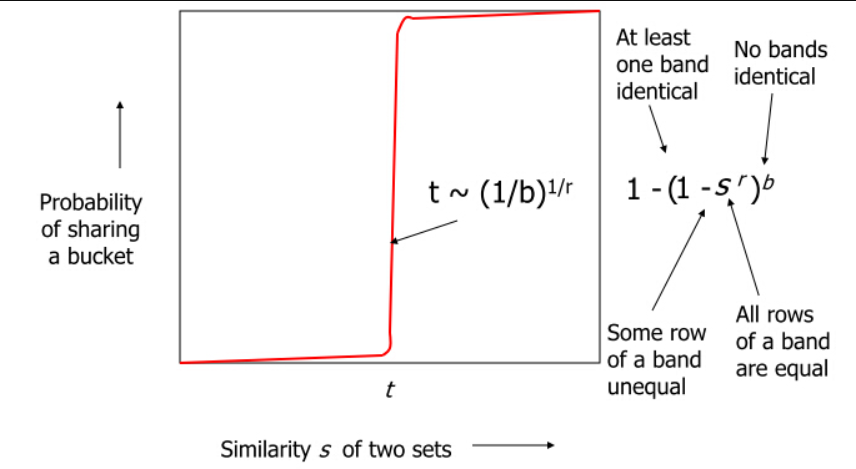
\includegraphics[width=5in]{img/img1.png}
    \caption{$s$与$Pr$关系图}
\end{figure}
由图像我们可知,当两个用户喜爱歌曲的相似度超过阈值t时,会有极大的概率使得至少一个brand内两个用户对应的hash值相同。
因此我们可以认为同一个桶内的元素对应的用户喜爱歌曲的相似度是超过阈值$t$的。

而我们可以通过参数的设置来设置阈值:
$$S(t) = (\frac{1}{B})^{\frac{1}{r}}$$


\paragraph{2.ppt1}~{}

设$\epsilon$为假阳性,假阳性是指$x \notin S$但$h(x)=h(x_i)$对某个$i$成立。

$$
\begin{aligned}
    Pr[\epsilon] &= Pr[\bigcup_{i=1}^{m} h(x) = h(x_i)] \\
    &= 1-Pr[\bigcap_{i=1}^{m} h(x) \ne h(x_i)]\\
    &= 1-\prod_{i=1}^{m} Pr[h(x) \ne h(x_i)]\\
    &= 1-(1-\frac{1}{C_b^k})^m
\end{aligned}
$$

\paragraph{2.ppt2}~{}
\subparagraph{随机投掷计算$\pi$}

假设投掷$n$次,共有$k$个落入圆中,则落入圆中的概率$p$为
$$
p = \frac{k}{n} \approx \frac{\pi r^2}{4r^2} = \frac{\pi}{4}
$$
$$
\pi = \frac{4k}{n}
$$
现在我们估计$Pr(\pi \notin [\frac{4k}{n}-\delta,\frac{4k}{n}+\delta])$
$$
\begin{aligned}
    Pr(\pi \notin [\frac{4k}{n}-\delta,\frac{4k}{n}+\delta]) 
   &= Pr[p < \frac{k}{n}-\frac{\delta}{4}] + Pr[p>\frac{k}{n}+\frac{\delta}{4}] \\ 
   &= Pr[np < k-\frac{\delta n}{4}] + Pr[np>k+\frac{\delta n}{4}] \\ 
   &= Pr[E(k) < k-\frac{\delta n}{4}] + Pr[E(k)>k+\frac{\delta n}{4}] \\ 
   &= Pr[k > E(k)+\frac{\delta n}{4}] + Pr[k < E(k)-\frac{\delta n}{4}] \\ 
   &= Pr[k > E(k)(1+\frac{\delta}{4p})] + Pr[k < E(k)(1-\frac{\delta}{4p})] \\ 
   &< exp(\frac{-E(k)(\frac{\delta}{4p})^2}{3}) + exp(\frac{-E(k)(\frac{\delta}{4p})^2}{2}) \\
   &= exp(\frac{-np(\frac{\delta}{4p})^2}{3}) + exp(\frac{-np(\frac{\delta}{4p})^2}{2})\\
   &\le exp(\frac{-n\delta^2}{48p}) + exp(\frac{-n\delta ^2}{32p})\\
   &< exp(\frac{-n\delta^2}{48}) + exp(\frac{-n\delta ^2}{32})
\end{aligned}
$$
则有
$$
Pr(\pi \in [\frac{4k}{n}-\delta,\frac{4k}{n}+\delta]) > 1 - exp(-n\frac{\delta^2}{48}) - exp(-n\frac{\delta ^2}{32})
$$
置信区间为$[\frac{4k}{n}-\delta,\frac{4k}{n}+\delta]$,置信度大于$1 - exp(-n\frac{\delta^2}{48}) - exp(-n\frac{\delta ^2}{32})$
\end{document}